
\subsubsection{Prijem i rapoređivanje dostiglih namirnica}
%\begin{figure}[H]
%	\begin{center}
	%	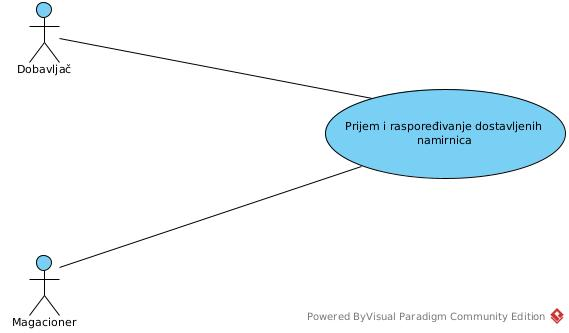
\includegraphics[width=\textwidth]{uc_receiving_groceries}
	%	\caption{Dijagram slučaja upotrebe prijema i raspoređivanja dostiglih namirnica}
%	\end{center}
%\end{figure}
	\begin{itemize}
		\item{Kratak opis:} 
		\begin{itemize}
			\item{Magacioner prihvata dostigle namirnice i raspoređuje ih u magacinu}
		\end{itemize}
		\item{Učesnici:} 
		\begin{itemize}
			\item{Magacioner}
	
		\end{itemize}		
		
		\item{Preduslovi:}
		\begin{itemize}
			\item{Magacioner je prijavljen na sistem.}
		\end{itemize}
		
		\item{Postuslovi:}
		\begin{itemize}
			\item{Sve dostigle namirnice su raspoređene u magacinu i baza podataka je ažurirana.}
		\end{itemize}
		
		\item{Osnovni tok:}
		\begin{enumerate}
			\item{Sistem obaveštava magacionera da je došlo do izmene spiska zakazanih isporuka.}
			\item{Magacioner proverava spisak zakazanih isporuka.}
			\item{Snabdevač isporučuje naručene namirnice do magacina.}
			\item{Magacioner proverava spisak dostiglih namirnica i njihovu količinu sa listom poručenih namirnica.}
			\item{Magacioner raspoređuje namirnice po magacinu.}
			\item{Magacioner beleži u sistemu da je završen prijem namirnica i spisak primljenih namirnica.}
			\item{Sistem ažurira bazu podataka u skladu sa spiskom primljenih namirnica.}
		\end{enumerate}
		
		\item{Alternativni tok:}
			\begin{enumerate}
				\item[4.a] {Magacioner vrši evidenciju namirnica koje se ne poklapaju na spiskovima i kako se ne poklapaju. Magacioner preuzima samo namirnice koje se poklapaju na spiskovima i u potrebnoj količini ili manjoj. Slučaj upotrebe se nastavlja od koraka 5.}
			\end{enumerate}
		\item{Dodatne informacije}
			\begin{itemize}
				\item{Informacije o datumu i vremenu isporuke, koji od snabdevača isporučuje namirnice, koje i u kojoj količini, se nalaze na spisku zakazanih isporuka za svaku od planiranih isporuka.}
			\end{itemize}
	\end{itemize}
\begin{figure}[H]
	\begin{center}
		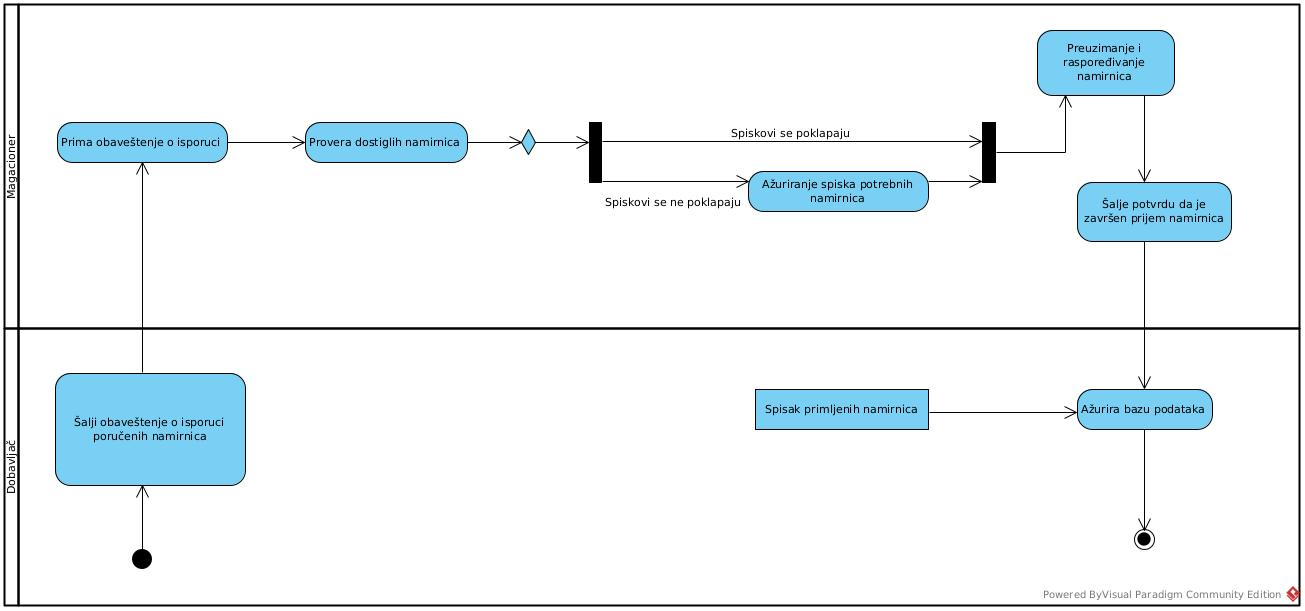
\includegraphics[width=\textwidth]{activity_receiving_groceries}
		\caption{Dijagram aktivnosti prijema i raspoređivanja dostiglih namirnica}
	\end{center}
\end{figure}
